\documentclass{article}
\renewcommand{\rmdefault}{psbx}
\usepackage[utf8]{inputenc}
\usepackage[T1]{fontenc}
\usepackage{textcomp}
\usepackage{eulervm}
\usepackage{amsmath}
\usepackage{amssymb}
\usepackage{graphicx}

\setlength{\textwidth}{160mm}
\setlength{\oddsidemargin}{0mm}
\setlength{\parindent}{0 mm}

\title{Propagating state distributions: \texttt{prop}}
\author{Carl Edward Rasmussen}
\date{December 26th, 2011}

\begin{document}

\maketitle

\begin{abstract}
This is a short documentation of \texttt{prop.m}.
\end{abstract}

At time $t$ the \emph{state distribution} consists of two copies of
the representation, the actual state, $s(t)$, and the \emph{forward
  predicted belief state}, $r(t)$. These are jointly Gaussian
\[
\left[\!\!\begin{array}{c}s(t)\\r(t)\end{array}\!\!\right]\;\sim\;
{\cal N}\left(\left[\!\!\begin{array}{c}\mu_s\\ \mu_r\end{array}\!\!\right],\;
\left[\!\!\begin{array}{cc}\Sigma_s&\Sigma_c\\ \Sigma_c^\top&\Sigma_r\end{array}\!\!\right]\right).
\]

The belief state, $b(t)$, is computed by combining the noisy actual
state ${\cal N}(\mu_s,\Sigma_y=\Sigma_s+\Sigma_n)$ with $r(t)$ using a
convex combination where each mean is weighted by its precision. Note,
that this only corresponds to the Bayesian posterior if $s(t)$ and
$r(t)$ are uncorrelated.
\[
\begin{split}
\mu_b\;&=\;\big(\Sigma_s^{-1}+\Sigma_r^{-1}\big)^{-1}\big(\Sigma_s^{-1}\mu_s+\Sigma_r^{-1}\mu_r\big)
\;=\;Z_r\mu_s+Z_n\mu_r,\\
\Sigma_b\;&=\;Z_r(\Sigma_s+\Sigma_n)Z_r^\top + Z_n\Sigma_rZ_n^\top +
 Z_r\Sigma_cZ_n^\top + Z_n\Sigma_c^\top Z_r^\top,
\end{split}
\]
where we have defined $Z_r=\Sigma_r(\Sigma_s+\Sigma_r)^{-1}$ and
$Z_n=\Sigma_n(\Sigma_s+\Sigma_r)^{-1}$.

\begin{figure}[ht]
\centerline{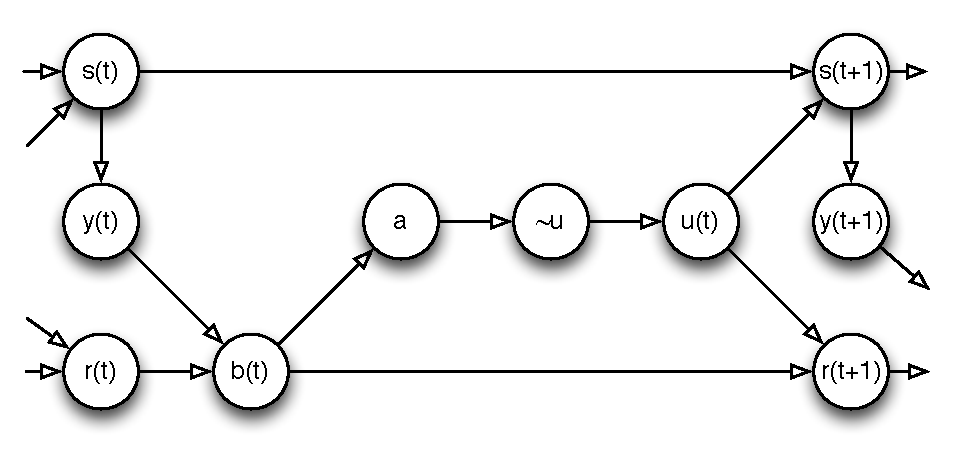
\includegraphics[width=0.8\textwidth]{prop1.pdf}}
\caption{Graphical model representing the time evolution of the state $s$
  and belief-state $b$.}
\end{figure}

\begin{figure}[ht]
\centerline{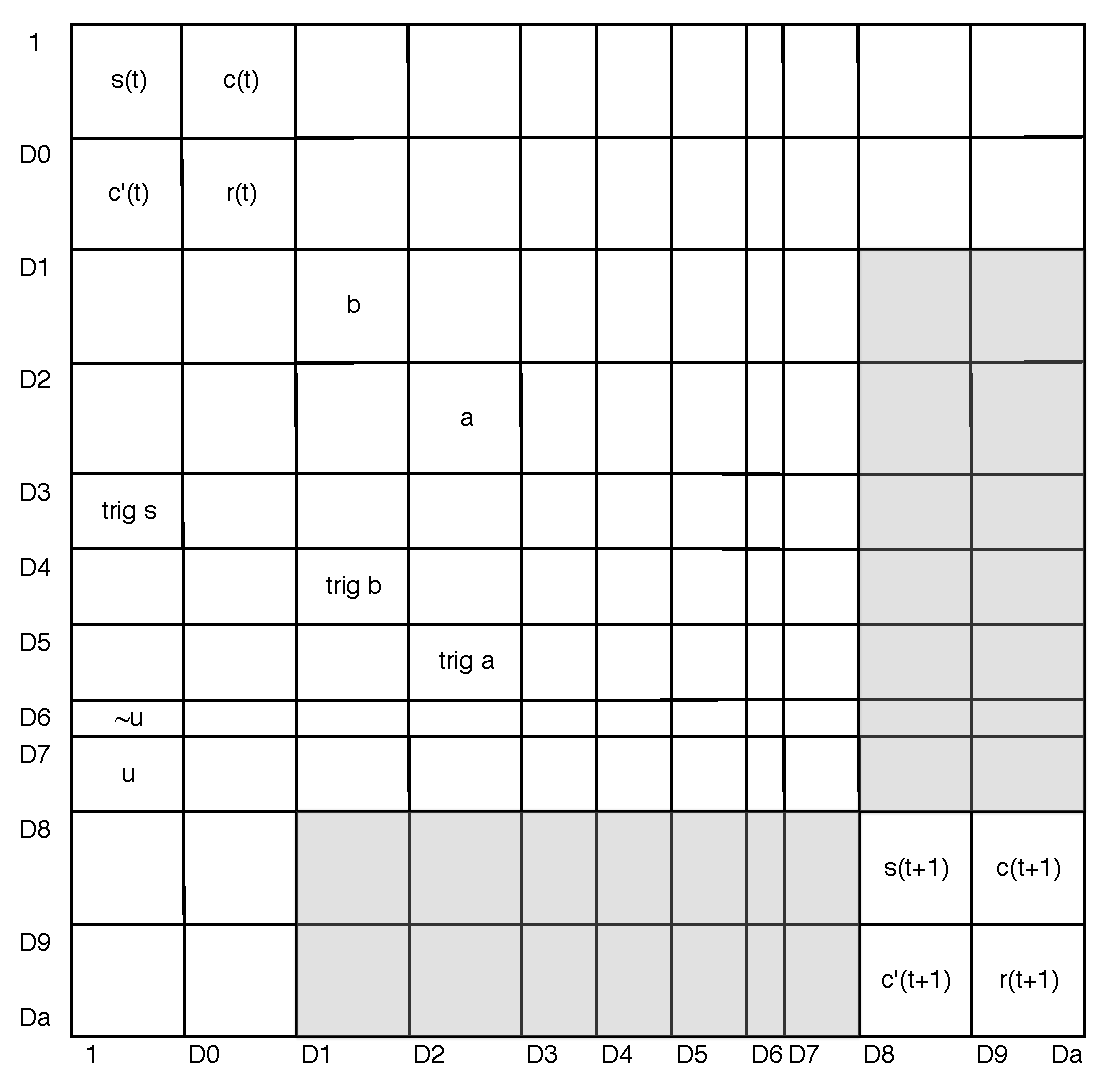
\includegraphics[width=0.8\textwidth]{prop2.pdf}}
\caption{Diagram showing the memory layout for the covariance matrix
  associated with a single forward propagation. The mean vector uses a
similar ordering. Shaded variables are never computed.}
\end{figure}





\end{document} 